%%%%%%%%%%%%%%%%%%%%%%%%%%%%%%%%%%%%%%%%%%%%%%%%%%%%%%%%%%%%
%%  This Beamer template was created by Cameron Bracken.
%%  Anyone can freely use or modify it for any purpose
%%  without attribution.
%%
%%  Last Modified: January 9, 2009
%%

\documentclass[xcolor=x11names,
								compress,
								aspectratio=1610]{beamer}
\usepackage{etex}

%% General document %%%%%%%%%%%%%%%%%%%%%%%%%%%%%%%%%%
\usepackage[utf8]{inputenc}
\usepackage[T1]{fontenc}
\usepackage[catalan]{babel}
\renewcommand*{\ttdefault}{beramono}
\usepackage{color}
\usepackage{graphicx}
\DeclareGraphicsExtensions{.pdf,.png,.jpg}
\graphicspath{{../memoir/img/}}
\usepackage{tikz}
\usetikzlibrary{shapes,arrows}
\usetikzlibrary{automata}
\usepackage{tikz-qtree}
\usetikzlibrary{arrows.meta}
\usetikzlibrary{decorations.pathreplacing}
\usepackage{amsmath,amsfonts,amssymb,amsthm,mathtools}
\newcommand{\mt}[1]{\texttt{#1}}
\DeclareMathSymbol{\mlq}{\mathord}{operators}{``}
\DeclareMathSymbol{\mrq}{\mathord}{operators}{`'}
\theoremstyle{definition}% <name>
\usepackage{booktabs}
\usepackage{minted}
\usemintedstyle{trac}
\definecolor{mintedbg}{rgb}{0.95, 0.95, 0.95}
\renewcommand{\theFancyVerbLine}{
	\scriptsize{\texttt{\arabic{FancyVerbLine}}}
}
\usepackage{siunitx}
\usepackage{framed}
\definecolor{shadecolor}{rgb}{0.95,0.95,0.95}
%%%%%%%%%%%%%%%%%%%%%%%%%%%%%%%%%%%%%%%%%%%%%%%%%%%%%%


%% Beamer Layout %%%%%%%%%%%%%%%%%%%%%%%%%%%%%%%%%%
\useoutertheme[subsection=false,shadow]{miniframes}
\useinnertheme{default}
\usefonttheme{serif}
\usepackage{palatino}

\setbeamerfont{title like}{shape=\scshape}
\setbeamerfont{frametitle}{shape=\scshape}

\setbeamercolor*{lower separation line head}{bg=DeepSkyBlue4} 
\setbeamercolor*{normal text}{fg=black,bg=white} 
\setbeamercolor*{alerted text}{fg=red} 
\setbeamercolor*{example text}{fg=black} 
\setbeamercolor*{structure}{fg=black} 
 
\setbeamercolor*{palette tertiary}{fg=black,bg=black!10} 
\setbeamercolor*{palette quaternary}{fg=black,bg=black!10} 

\renewcommand{\(}{\begin{columns}}
\renewcommand{\)}{\end{columns}}
\newcommand{\<}[1]{\begin{column}{#1}}
\renewcommand{\>}{\end{column}}
%%%%%%%%%%%%%%%%%%%%%%%%%%%%%%%%%%%%%%%%%%%%%%%%%%

\newsavebox{\longestsec}

\begin{document}


%%%%%%%%%%%%%%%%%%%%%%%%%%%%%%%%%%%%%%%%%%%%%%%%%%%%%%
%%%%%%%%%%%%%%%%%%%%%%%%%%%%%%%%%%%%%%%%%%%%%%%%%%%%%%
\begin{frame}
\title{Patrons de Connexió al CV de la UOC}
%\subtitle{SUBTITLE}
\author{
	Armand Adroher Salvia\\
	{\it UOC - TFG - GEI - EDM\&LA}\\
}
\date{
	26 de gener del 2015
}
\titlepage
\end{frame}

%%%%%%%%%%%%%%%%%%%%%%%%%%%%%%%%%%%%%%%%%%%%%%%%%%%%%%
%%%%%%%%%%%%%%%%%%%%%%%%%%%%%%%%%%%%%%%%%%%%%%%%%%%%%%
\begin{frame}{}
%\begin{center}
\begin{lrbox}{\longestsec}{\scshape Abstracció}\end{lrbox}% Capture longest title
  \setlength{\leftskip}{\dimexpr.45\textwidth-.4\wd\longestsec\relax}
\tableofcontents[hideallsubsections]
%\end{center}
\end{frame}

\section{\scshape Objectius}

	\subsection{Dades rebudes}
	\begin{frame}[fragile]{Dades rebudes}
	
		\begin{itemize}
		\item Camps
		$$
			\langle \mt{user\_id}, \mt{session\_start}, \mt{last\_request}, \mt{session\_expiration} \rangle
		$$
		\usemintedstyle{trac}
\begin{minted}[linenos=true,
                bgcolor=mintedbg,
                fontfamily=tt,
                %numbersep=-2\tabcolsep,
                numbersep=.5pt,
                gobble=0,
                fontsize=\scriptsize,
%                frame=lines,
                framesep=\baselineskip,
%                xleftmargin=2\tabcolsep,
                baselinestretch=0.75,
                tabsize=2
								]{text}
7149084242663;18/09/2013 00:00:03;18/09/2013 00:57:28;18/09/2013 02:04:32
6059394219413;18/09/2013 00:00:04;18/09/2013 00:00:15;18/09/2013 01:07:21
4139154106177;18/09/2013 00:00:07;18/09/2013 00:31:29;18/09/2013 01:39:07
 858883854230;18/09/2013 00:00:07;18/09/2013 00:00:12;18/09/2013 01:07:21
\end{minted}

	\item Dimensions
	
	\begin{align*}
	\#\langle \ldots \rangle & \approx \SI{8}{M}  
	& 
	\min(\texttt{session\_start}) & \in \texttt{2013-09-18} \\
	\# \mt{user\_id} & \approx 75\text{K} 
	&  
	\max(\texttt{session\_expiration}) & \in \texttt{2014-01-15} 
	\end{align*}

\end{itemize}

\end{frame}
	
	\subsection{Model de dades}
	\begin{frame}{Model de dades}
	\begin{itemize}
	\item Sessions
%	\vspace{0.5 cm}
	\begin{center}
		
		\begin{tikzpicture}[scale=1.6]

\tikzstyle{every node}=[font=\scriptsize]

\draw[->] (0.5,2) node [left] {$t$} -- (8.5,2);
\draw[|-{Rays[]}, thick] 
			(1,3) node [above=3pt] 
				{\texttt{session\_start}} 
	-- 	(3,3) node [above=3pt] 
				{\texttt{central\_activity\_point}};
\draw[thick] (2.9,3) -- (5,3);
\draw[|-|, dashed, thick] 
			(5,3) node [above=3pt] 
					{\texttt{last\_request}} 
	-- 	(7,3) node [above=3pt] 
					{\texttt{session\_expiration}};

\draw[decorate,decoration={brace, mirror}]
			(1,2.75) -- (5,2.75) 
				node [midway,below] 
				{\texttt{activity\_duration}};
\draw[decorate,decoration={brace, mirror}]
			(5,2.75) -- (7,2.75) 
				node [midway,below] 
				{\texttt{inactivity\_duration}};
%\draw plot[mark=|] coordinates {(1,3) (3,3) (5,3) (7,3)};
%\draw plot[mark=|] coordinates {(1,3) (3,3) (5,3) (7,3)}; 
\end{tikzpicture}

		\end{center}
		\item Usuaris
		\vspace{.5cm}
		\begin{center}
\begin{tikzpicture}[node distance=4cm]
\tikzstyle{every node}=[font=\scriptsize]
\node (student) [draw, inner sep=5pt] {\texttt{user}};
\node (session) [draw, right of=student, inner sep=5pt] {\texttt{session}};
\draw (student) -- node [very near start, above] {\texttt{1}} node [very near end, above] {\texttt{1-*}}(session);
\end{tikzpicture}
\end{center}
\vspace{.5cm}

		\end{itemize}
	\end{frame}	
	
\subsection{Anomalies}
\begin{frame}{Anomalies}
\begin{itemize}
	\item Subsessions negatives
	$$
	l(\mt{activity\_duration}) < \SI{0}{s} \vee 
    l(\mt{inactivity\_duration}) < \SI{0}{s}
	$$
	\item Solapament de sessions
	\vspace{.5cm}
	\begin{center}
\begin{tikzpicture}[scale=0.5]

\tikzstyle{every node}=[font=\scriptsize]

\node [draw] at (0,5) {\texttt{user}$_i$};

\draw[->] (0,0) node [left] {$t$} -- (20,0);

% 1
\draw[|-, thick] (1,3) -- (5,3);
\draw[|-|, dashed, thick] (5,3) -- 	(7,3);

% 2
\draw[|-, thick] (5.5,1.5) -- (8.5,1.5);
\draw[|-|, dashed, thick] (8.5,1.5) -- 	(9,1.5);

% 3
\draw[|-, thick] (9.5,3) -- (10.5,3);
\draw[|-|, dashed, thick] (10.5,3) -- 	(15,3);

% 4
\draw[|-, thick] (11,1.5) -- (13.75,1.5);
\draw[|-|, dashed, thick] (13.75,1.5) -- 	(14.75,1.5);

% 5
\draw[|-, thick] (16,1.5) -- (17,1.5);
\draw[|-|, dashed, thick] (17,1.5) -- 	(19.5,1.5);

\end{tikzpicture}
\end{center}

\end{itemize}
\end{frame}

\subsection{Objectiu general}
\begin{frame}{Objectiu general}
\begin{itemize}
\item Posar en pràctica la EDM\&LA
	\begin{shaded}
	\vspace{1cm}
	\begin{itemize}
		\item \large{KDD i ML per a millorar els processos d'aprenentatge}
		\vspace{1cm}
		\item \large{En el context del CV de la UOC}
	\end{itemize}
	\vspace{1cm}
	\end{shaded}
\end{itemize}
\end{frame}

\subsection{Dificultats}
\begin{frame}{Dificultats}

\begin{itemize}
	\item Procés de generació de les dades
		\begin{itemize}
		\item Registre (\emph{log}) de servidor?
		\item Agregat en lots (\emph{batch}) o en temps real?
		\end{itemize}
	\item Tipus d'usuaris
		\begin{itemize}
		\item Estudiants?
		\item Consultors, PAS, \emph{alumni}, etc.?
		\end{itemize}
	\item Comportament de l'usuari
		\begin{itemize}
		\item Accions en \mt{session\_start} i \mt{last\_request}
		\item Què més?
		\end{itemize}
\end{itemize}

\end{frame}

\section{\scshape Abstracció}
	\subsection{Distribució de valors}
	\begin{frame}{Distribució de valors}
	\begin{itemize}
		\item Patró general de comportament
		\item Consonància amb el sentit comú
	\end{itemize}
	\begin{columns}[onlytextwidth]
		\begin{column}{.5\textwidth}
		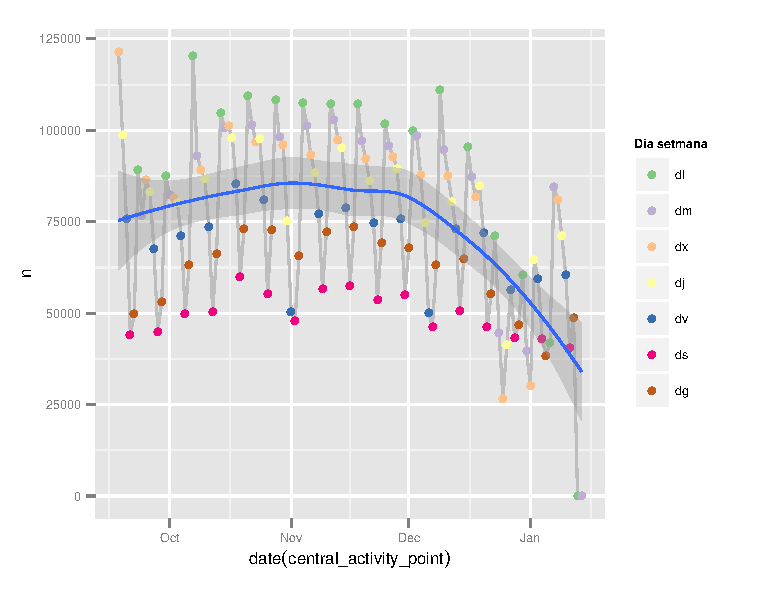
\includegraphics[width = \textwidth]{n_sessions_pday_scatter}
		\end{column}
		\begin{column}{.5\textwidth}
		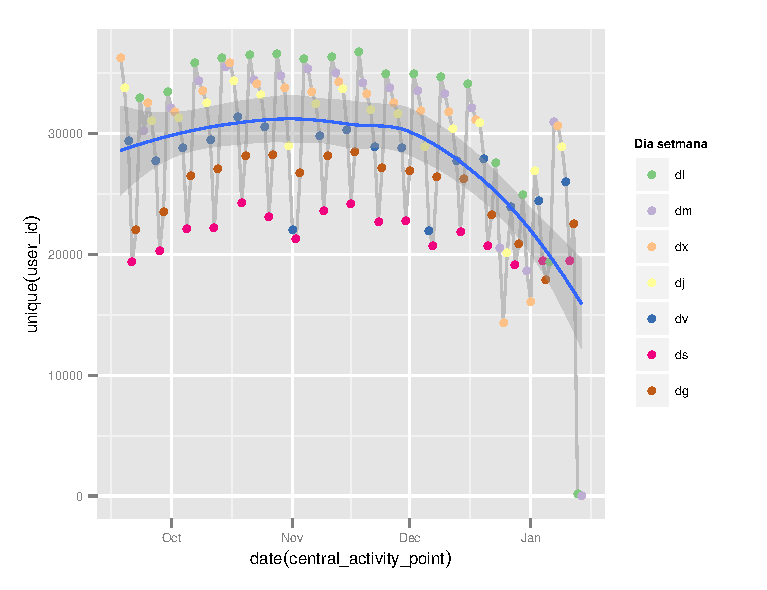
\includegraphics[width = \textwidth]{n_users_pday_scatter}
		\end{column}
	\end{columns}
	\end{frame}
	
	\subsection{Dispersió de valors}
	\begin{frame}{Dispersió de valors}
	\begin{itemize}
		\item Molts valors petits
		\item Molt pocs valors molt grans
	\end{itemize}
	\begin{columns}[onlytextwidth]
		\begin{column}{.5\textwidth}
		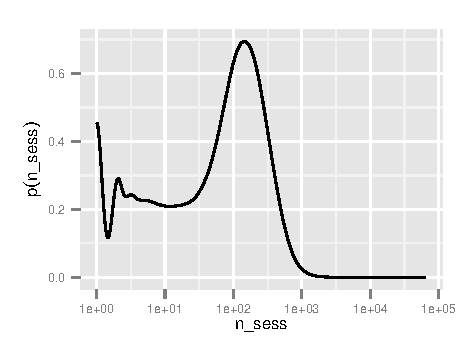
\includegraphics[width = \textwidth]{user_n_sessions_density_line_log}
		\end{column}
		\begin{column}{.5\textwidth}
		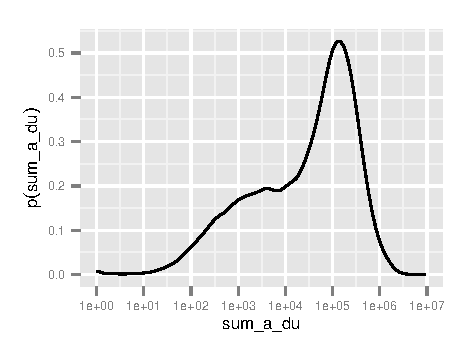
\includegraphics[width = \textwidth]{user_sum_activity_duration_density_line_log}
		\end{column}
	\end{columns}
	\end{frame}
	
	\subsection{Superació de les dificultats}
		\begin{frame}{Superació de les dificultats}
		\begin{columns}[onlytextwidth]
  		\begin{column}{.5\textwidth}
				\begin{itemize}
				\item Limitar-se a la informació rebuda
				\item Inici $\rightarrow$ final de la interacció
				\item Presència per unitat de temps
				\end{itemize}
			\end{column}
  		\begin{column}{.5\textwidth}
  		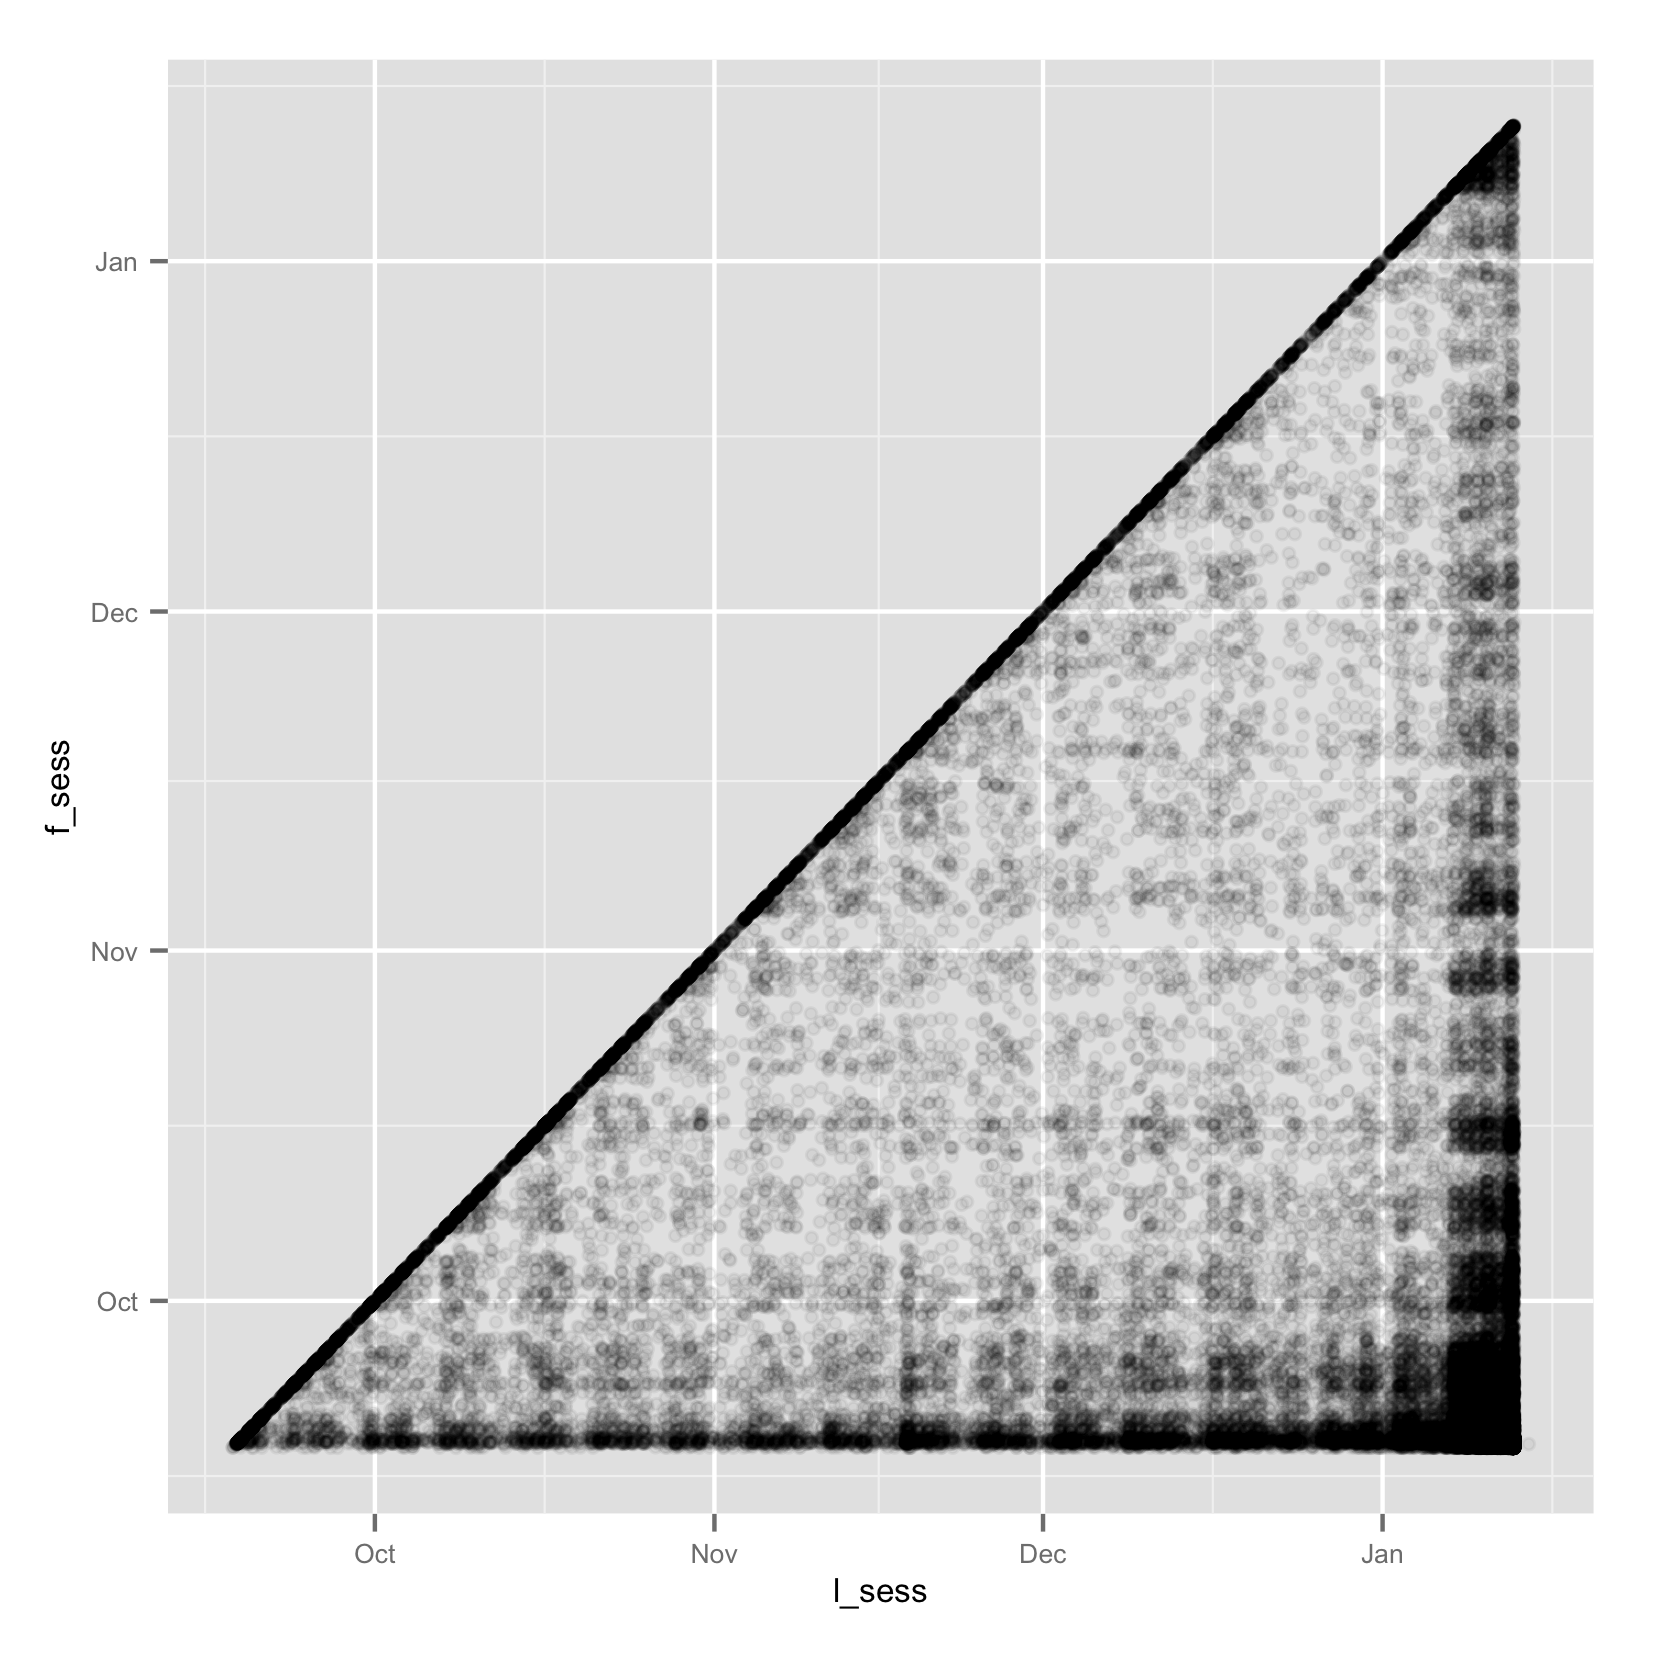
\includegraphics[width = \textwidth]{user_first_last_scatter}
  		\end{column}
		\end{columns}
	\end{frame}

\subsection{Nous atributs}
\begin{frame}{Nous atributs}
	\begin{itemize}
	\item Discretització temporal
	\begin{align*}
		\mt{semester} & = I_0, \ldots, I_m
		&
		t_0 & \in I_0 
		& 
		I_j = [t_0 + dj, t_0 + d(j+1)]
	\end{align*}
	\item Atributs booleans
	\begin{align*}
		\mt{user}_i & = \langle \mt{id}_i, a_{i,0},\ldots,a_{i,m} \rangle
		\quad (a_{i,j}  \in \{0,1\}) \\
		a_{i,j} & = \begin{cases}
					1 \text{ si } \{v \in \mt{sessions}_i : \phi(v,j)  \} \neq \emptyset   \\
					0 \text{ altrament}
					\end{cases} \\
		\phi(v,j) & = (v.\mt{session\_start} \leq t_0 + d(j+1)) \wedge (t_0 + dj \leq v.\mt{last\_request})
	\end{align*}
	\item Dos valors de $d$
	\begin{align*}
	d & \leftarrow 1\text{ dia} & d & \leftarrow 1\text{ setmana}
	\end{align*}
	\end{itemize}
\end{frame}

\subsection{Nous objectes}
\begin{frame}{Nous objectes}
	\begin{itemize}
	\item Usuari $i$-èssim $\mapsto$ seqüència de valors booleans
	\end{itemize}
%	\vspace{1cm}
	\begin{center}
	\begin{tikzpicture}
	\node (user) at (-2.5,0) {$\mt{user}_i:$};
%	\node (ldots) at (-1,0) {$\ldots$};
	\node[draw, rectangle] (s_0) at (0,0) {0};
	\node[draw, rectangle] (s_1) at (0.5,0) {0};
	\node[draw, rectangle] (s_2) at (1,0) {1};
	\node (cdots) at (2,0) {$\ldots$};
	\node[draw, rectangle] (s_3) at (3,0) {0};
	\node[draw, rectangle] (s_4) at (3.5,0) {1};
	
	\draw[decorate,decoration={brace, mirror}] 
			(-.2,-.4)  -- 	(.2,-.4) 
				node [midway,below] {$I_0$};
	\draw[decorate,decoration={brace, mirror}] 
			(.3,-.4)  -- 	(.7,-.4) 
				node [midway,below] {$I_1$};
	\draw[decorate,decoration={brace, mirror}] 
			(.8,-.4)  -- 	(1.2,-.4) 
				node [midway,below] {$I_2$};
	\draw[decorate,decoration={brace, mirror}] 
			(2.8,-.4)  -- 	(3.2,-.4) 
				node [midway,below, xshift=-.6] {$I_{m-1}$};
	\draw[decorate,decoration={brace, mirror}] 
			(3.3,-.4)  -- 	(3.7,-.4) 
				node [midway,below] {$I_m$};
				
	\draw[|-] (user) -- (s_0);
	\draw[-] (s_0) -- (s_1);
	\draw[-] (s_1) -- (s_2);
	\draw[-] (s_2) -- (cdots);
	\draw[-] (cdots) -- (s_3);
	\draw[-] (s_3) -- (s_4);
	\draw[->] (s_4) -- (6.5,0) node[near end, below] {$t$};
	
	\node[above of=s_0, xshift=-.6] (a_0) {$a_{i,0}$};
	\node[above of=s_1] (a_1) {$a_{i,1}$};
	\node[above of=s_2, xshift=.6] (a_2) {$a_{i,2}$};
	\node[above of=s_3, xshift=-1.6] (a_3) {$a_{i,m-1}$};
	\node[above of=s_4, xshift=5] (a_4) {$a_{i,m}$};
	
	\draw[->] (s_0) -- (a_0);
	\draw[->] (s_1) -- (a_1);
	\draw[->] (s_2) -- (a_2);
	\draw[->] (s_3) -- (a_3);
	\draw[->] (s_4) -- (a_4);
	
	\end{tikzpicture}
	\end{center}
	\begin{itemize}
	\item $a_{i,j} = 1$ si i només si l'usuari $i$-èssim \emph{ha estat present al CV} durant $I_j$
	\end{itemize}
\end{frame}

\section{\scshape Agregació}
\subsection{k-means}
\begin{frame}{k-means}
	\begin{columns}[onlytextwidth]
		\begin{column}{.5\textwidth}
		\begin{itemize}
  	\item $k$-means (\emph{Lloyd}) sobre 
		\begin{align*}
			a_{i,0},\ldots,a_{i,m} & \in \{0,1\}^{m+1}
%			&
%			S = \{s_1,\ldots,s_k\} \subset \mathcal{P(\mt{users})}
		\end{align*}
		\item Tipus de comportaments
		\begin{align*}
			\mu_1,\ldots,\mu_k & \Rightarrow \text{ caracterització}
		\end{align*}
  	\end{itemize}
		\begin{center}
		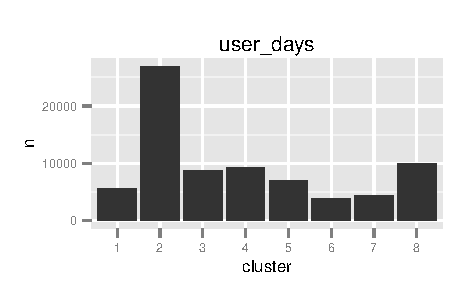
\includegraphics[width=\textwidth]{user_presence_8means_clusts}
		\end{center}
		\end{column}
		\begin{column}{.5\textwidth}
		\begin{itemize}
			\item Agregació jeràrquica sobre
				$$
				 \mu_1,\ldots,\mu_k
				$$
			\item Enllaç complet
			\end{itemize}
			\begin{center}
			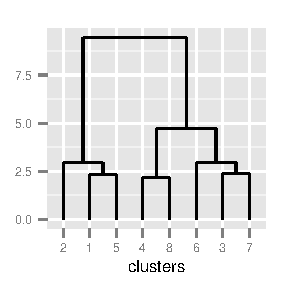
\includegraphics{presence_complete_dendrogram_8means_clusts}
			\end{center}
		\end{column}
	\end{columns}
\end{frame}

\subsection{Patrons}
\begin{frame}{Patrons}
	\begin{columns}[onlytextwidth]
		\begin{column}{.5\textwidth}
    	\begin{itemize}
    	\item Tipologia de comportaments
    	\end{itemize}
    		\begin{enumerate}[A.]
    		\item \textbf{Absents} $\{1,2,5\}$ (52.2\%)	
    			\begin{enumerate}[a.]
    			\item \textbf{Esporàdics} $\{2\}$
    			\item \textbf{Capbussadors} $\{1\}$
    			\item \textbf{Tímids} $\{5\}$
    			\end{enumerate}
    		\item \textbf{Presents} $\{3,4,6,7,8\}$ ($47.8\%$)
    			\begin{enumerate}[a.]	
    			\item \textbf{Endarrerits} $\{6\}$	
    			\item \textbf{Fatigats} $\{3\}$
    			\item \textbf{Setmanaris} $\{7\}$
    			\item \textbf{Persistents} $\{3,7\}$
    				\begin{enumerate}[i.]
    				\item \textbf{Dedicats} $\{8\}$
    				\item \textbf{Obsessionats} $\{4\}$ 
    				\end{enumerate} 
    			\end{enumerate}	
    		\end{enumerate}
		\end{column}
		\begin{column}{.5\textwidth}
		\begin{center}
		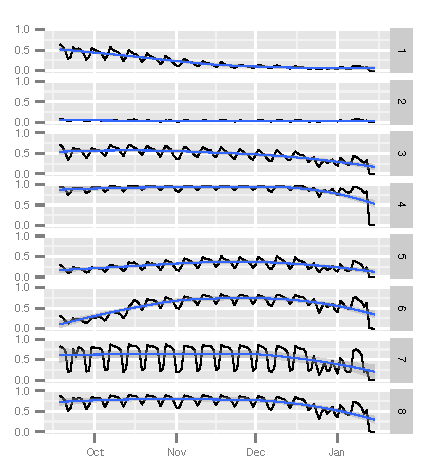
\includegraphics{presence_8_clust_pres}
		\end{center}	
		\end{column}
	\end{columns}
\end{frame}

\subsection{Limitacions}
\begin{frame}{Limitacions}
	\begin{columns}[onlytextwidth]
		\begin{column}{.5\textwidth}
			\begin{itemize}
			\item A partir de dades pobres
				$$
				P(a_{i,j}=1|\mt{user}_i \in \mt{students}) \quad ?
				$$
			\vspace{1cm}
			\item \emph{A posteriori}
				
				Després del final del semestre
				
				$\Rightarrow$ No es pot actuar en temps real

			\end{itemize}
		\end{column}
		\begin{column}{.5\textwidth}
			\begin{itemize}
			\item Prediccions poc significatives
			$$
				\kappa_i = \begin{cases}
						1 \text{ si } \mt{l\_sess}_i < Q_2(\mt{l\_sess}) \\
						0 \text{ altrament} 
					\end{cases} 
			$$
			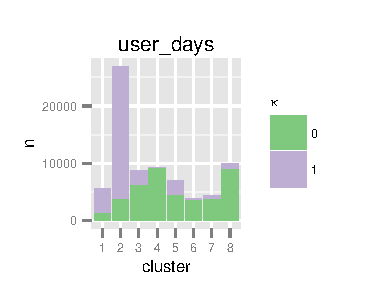
\includegraphics{user_presence_pred8means_clusts}	
			\end{itemize}
		\end{column}
	\end{columns}
	
\end{frame}

\section{\scshape Predicció}
\subsection{Cadenes de Markov}
\begin{frame}{Cadenes de Markov}
	\begin{columns}[onlytextwidth]
		\begin{column}{.5\textwidth}
			\begin{itemize}
			\item $a_0,\ldots,a_m$ seqüència d'estats $\{0,1\}$
			\begin{align*}
      	\mt{user}_1 \mapsto & \quad 00001011101001\ldots \\
      	 & \vdots \\
      	\mt{user}_n \mapsto & \quad \underbrace{11001010010101\ldots}_{m+1} 
      \end{align*}
      \item DTMC homogènia de grau 1
      \begin{center}
      \begin{tikzpicture}[node distance = 4cm]
      
      \node[state] (present) {$1$};
      \node[state, right of=present] (absent) {$0$};
      
      \path[->] (present) 	edge [bend left]		
      							node [above] {$P(0|1)$} (absent)
      						(absent) 	edge [bend left]		
      							node [below] {$P(1|0)$} (present)
      						(present) 	edge [loop left]		
      							node [left] {$P(1|1)$} (present)
      						(absent) 	edge [loop right]		
      							node [right] {$P(0|0)$} (absent);
      \end{tikzpicture}
      \end{center}
			\end{itemize}
			
		\end{column}
		\begin{column}{.5\textwidth}
			\begin{itemize}
			\item Representació de \mt{user}$_i$ 
			$$
      \begin{pmatrix}
      P(0|0) & P(1|0) \\
      P(0|1) & P(1|1)
      \end{pmatrix}
      = 
      \begin{pmatrix}
      1 - \alpha & \alpha \\
      1 - \beta & \beta
      \end{pmatrix}
      $$
      
      Paràmetres a estimar: $\alpha,\beta$
			\vspace{4.6cm}
			\end{itemize}
		\end{column}
	\end{columns}
\end{frame}

\subsection{Estimació per a DTMC}
\begin{frame}{Estimació per a DTMC}
	\begin{columns}[onlytextwidth]
		\begin{column}{.5\textwidth}
			\begin{itemize}
			\item Estimador $\widehat{p}_{x,y}$
			\begin{align*}
				x,y & \in \{0,1\} \\
				n_{x,y} & = \text{transicions } x \rightarrow y  \\
      	\widehat{p}_{x,y} & = \frac{n_{x,y}}{ \displaystyle \sum_{z \in \{0,1\}} n_{x,z}} \\ 
      \alpha & = \frac{n_{0,1}}{ \displaystyle \sum_{z \in \{0,1\}} n_{0,z}} \quad
      \beta  = \frac{n_{1,1}}{ \displaystyle \sum_{z \in \{0,1\}} n_{1,z}}
      \end{align*}
			\end{itemize}
		\end{column}
		\begin{column}{.5\textwidth}
			\begin{itemize}
			\item Resultats dispersos
			\end{itemize}
			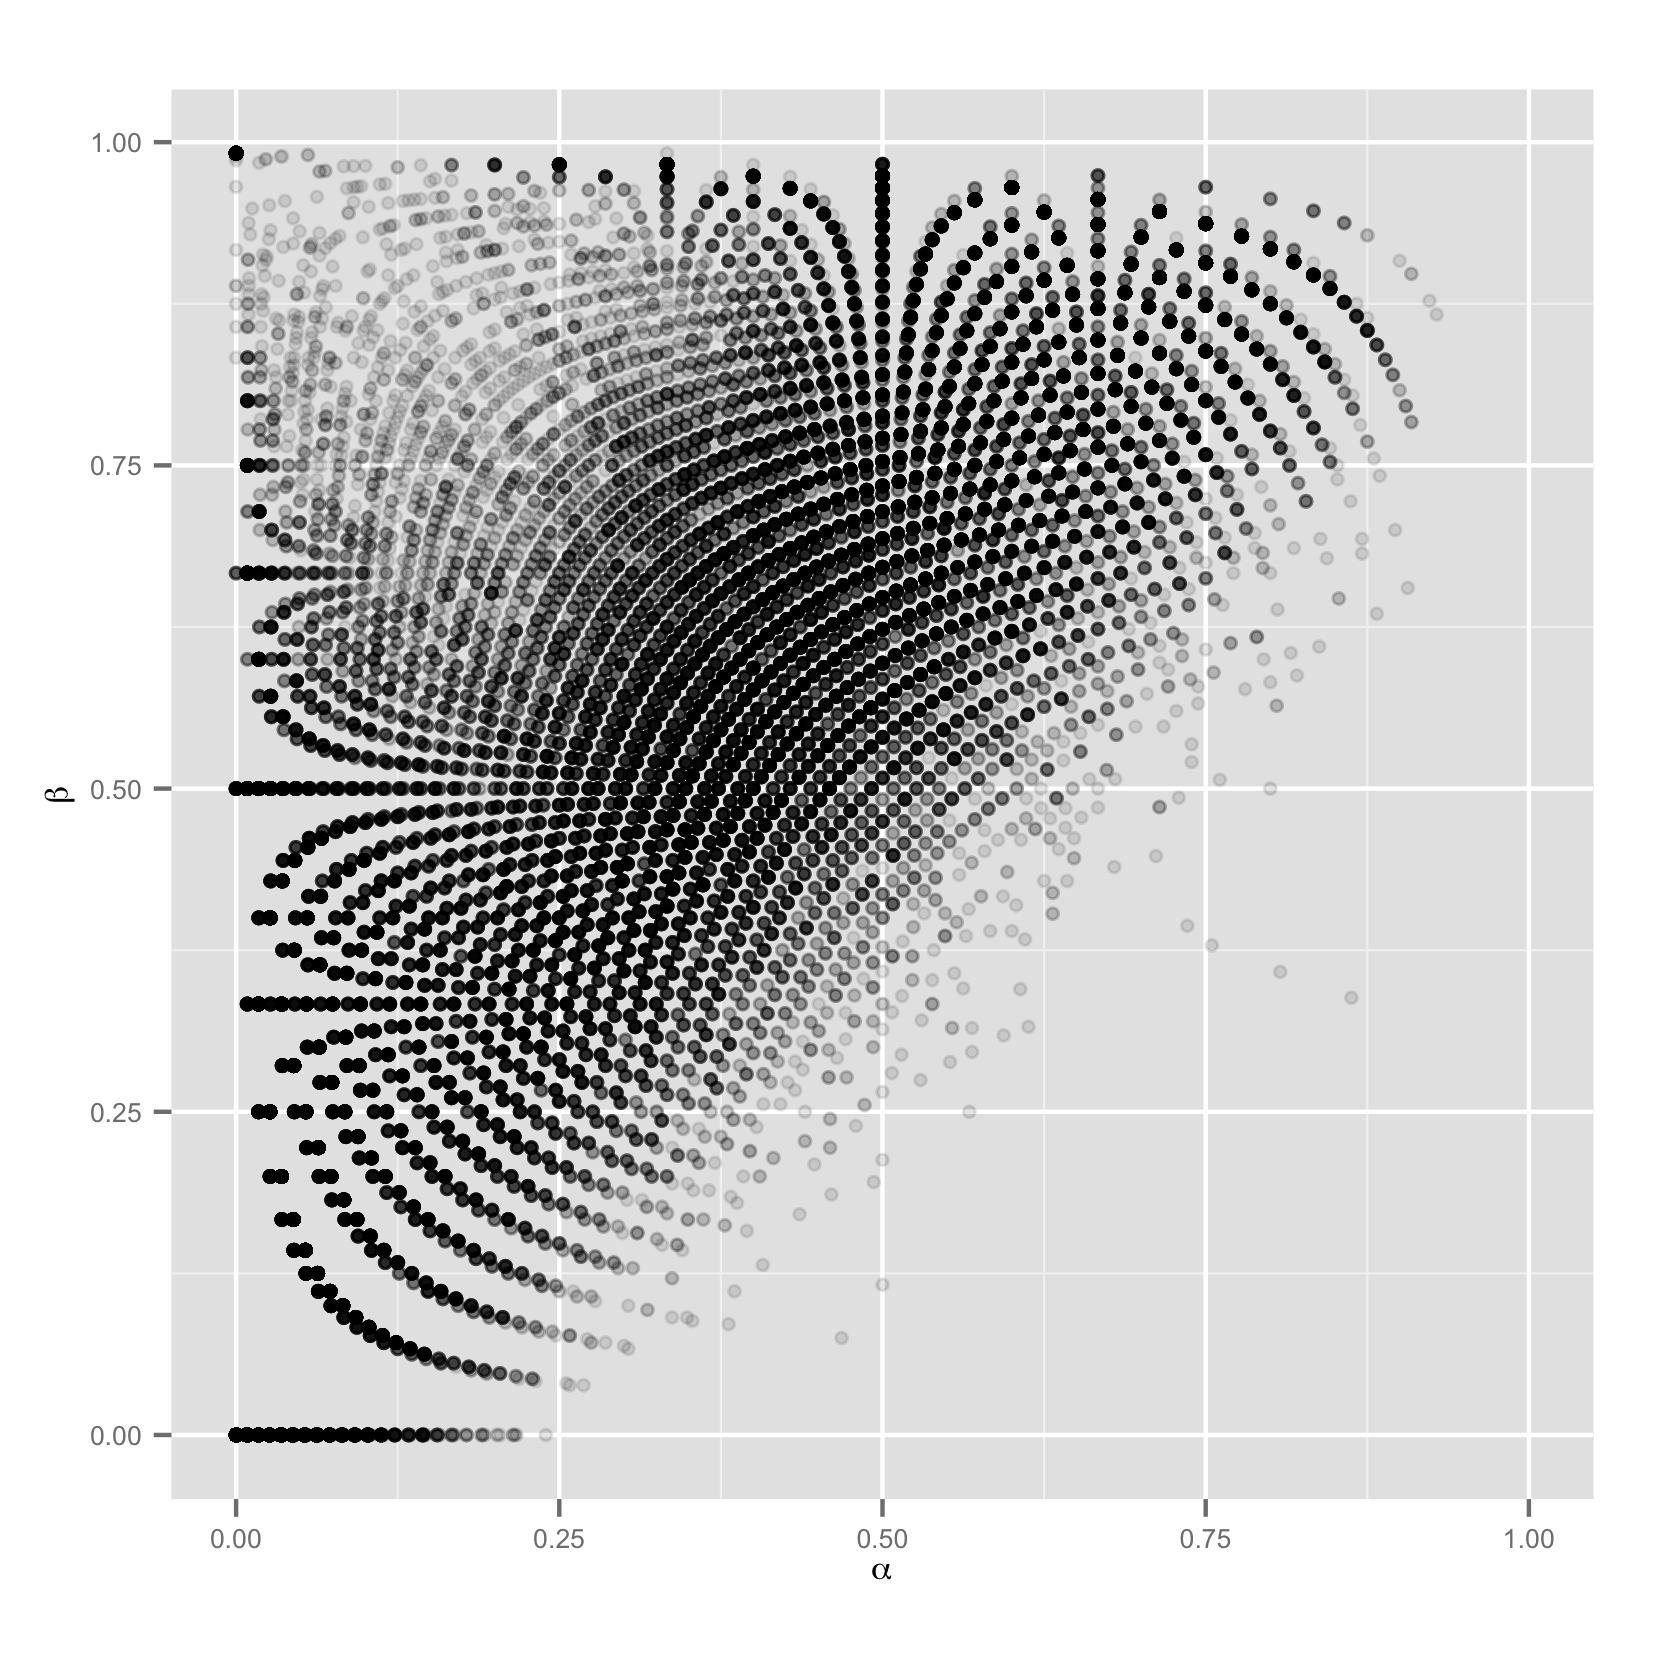
\includegraphics[width=.9\textwidth]{mc_params_days}
		\end{column}
	\end{columns}
\end{frame}

\subsection{Model ocult de Markov}
\begin{frame}{Model ocult de Markov}
	\begin{columns}[onlytextwidth]
		\begin{column}{.5\textwidth}
			\begin{itemize}
			\item Estats ocults $S = \{A,Q\}$
			\end{itemize}
			$$
			x_{i,j} = Q \Leftrightarrow \mt{user}_i \text{ ha abandonat el CV}
			$$
			\begin{itemize}
			\item Observacions $a_{i,j} \in \{0,1\}$
			\item Transicions
			$$
      \begin{pmatrix}
      P(Q|Q) & P(A|Q) \\
      P(Q|A) & P(A|A)
      \end{pmatrix}
      =
      \begin{pmatrix}
      1 & 0 \\
      1- \alpha & \alpha
      \end{pmatrix}
      $$
			\item Emissions
			$$
      \begin{pmatrix}
      P(0|Q) & P(1|Q) \\
      P(0|A) & P(1|A)
      \end{pmatrix}
      =
      \begin{pmatrix}
      1 & 0 \\
      1 - \beta & \beta
      \end{pmatrix}
      $$
			\end{itemize}
		\end{column}
		\begin{column}{.5\textwidth}
		\begin{center}
      \begin{tikzpicture}[node distance = 4cm, scale=.75]
      
      \node[state, above of=present] (active) {$A$};
      \node[state, above of=absent] (quit) {$Q$}; 
      
      \node[state] (present) {$1$};
      \node[state, right of=present] (absent) {$0$};
      
      \path[->] (active) 	edge [bend left]		
      							node [above] {$1 - \alpha$} (quit)
      						(quit) 	edge [bend left]		
      							node [below] {$0$} (active)
      						(active) 	edge [loop left]		
      							node [left] {$\alpha$} (active)
      						(quit) 	edge [loop right]		
      							node [right] {$1$} (quit);
      							
      \path[->] (active) edge [bend right] 
      							node [left] {$\beta$} (present)
      						(active) edge [bend right] 
      							node [below left] {$1 -\beta$} (absent)
      						(quit) edge [bend left]
      							node [below right] {$0$} (present)
      						(quit) edge [bend left]
      							node [right] {$1$} (absent);	
      							
      \draw[dashed] (-2,3.5) -- (7.5,3.5);						
      							
      \end{tikzpicture}
    \end{center}
		\end{column}
	\end{columns}
\end{frame}

\subsection{Estimació per a HMM}
\begin{frame}{Estimació per a HMM}
	\begin{columns}[onlytextwidth]
		\begin{column}{.5\textwidth}
			\begin{itemize}
			\item Per a $\alpha$, prenem $\lambda$ tal que $ Q_2(\mt{l\_sess}) \in I_\lambda$
			\begin{align*}
      \begin{pmatrix}
      P(Q) & P(A)
      \end{pmatrix}
      &
      \begin{pmatrix}
      P(Q|Q) & P(A|Q) \\
      P(Q|A) & P(A|A)
      \end{pmatrix}^\lambda
      \\
      = &
      \begin{pmatrix}
      0 & 1
      \end{pmatrix}
      \begin{pmatrix}
      1 & 0 \\
      1 - \alpha & \alpha
      \end{pmatrix}^\lambda
      \\
      = &
      \begin{pmatrix}
      1-\alpha^\lambda & \alpha^\lambda
      \end{pmatrix} \\
      \alpha^{\lambda} = \frac{1}{2} \quad \Rightarrow & \quad \alpha = \left(\frac{1}{2}\right)^{\frac{1}{\lambda}} \\
      \end{align*} 
			\end{itemize}
		\end{column}
		\begin{column}{.5\textwidth}
		\begin{itemize}
		\item Per a $\beta$, prenem $u$ tal que $\mt{user}_i.\mt{l\_sess} \in I_u$
		\begin{align*}
			\mt{user}_i.\mt{a\_rate} = & \frac{1}{u+1} \sum_{j = 0}^u a_{i,j} \\
			\beta = \frac{1}{|\mt{users}|} & \sum_{v \in \mt{users}} v.\mt{a\_rate}
		\end{align*}
		\vspace{1.9cm}
		\end{itemize}
		\end{column}
	\end{columns}
\end{frame}

\subsection{Predicció de l'abandonament}
\begin{frame}{Predicció de l'abandonament}
			\begin{itemize}
			\item En temps real
			
			Per a cada interval $I_j$ i cada usuari $i$-èssim
			
			\end{itemize}
			
			\begin{align*}
			\mt{viterbi} (HMM(\alpha, \beta), \langle a_{i,0},\ldots, a_{i,j}\rangle) \quad = & \quad \langle x_{i,0},\ldots, x_{i,j} \rangle \\ 
			\mt{user}_i \text{ ha abandonat }  \quad \Leftrightarrow & \quad x_{i,j} = Q
 			\end{align*}
			\begin{center}
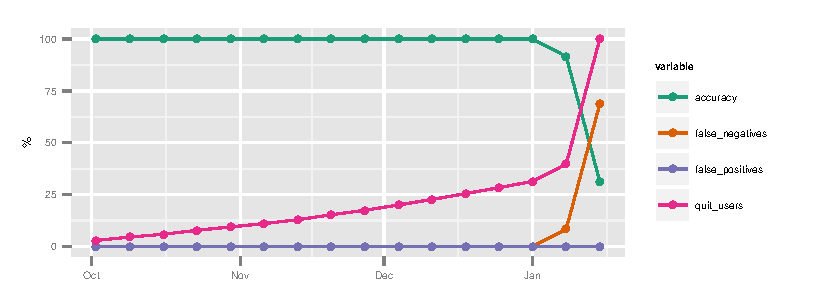
\includegraphics{hmm_weeks_confusion_m_day_pres}  
			\end{center}
\end{frame}

\section{\scshape Conclusions}
\subsection{Conclusions}
\begin{frame}{Conclusions}
	\begin{shaded}
	\begin{itemize}
		\item \large{
			La discretització en presència/absència per interval temporal és útil per a dotar de significat dades com aquestes.	
		}
		\vspace{1cm}
		\item \large{
			L'agregació per k-means permet fer un esbós \emph{a posteriori} de la tipologia d'usuaris segons el patró de connexió.
		}
		\vspace{1cm}
		\item \large{
			La predicció \emph{a priori} de l'abandonament del CV per mitjà de models ocults de Markov és eficaç en el cas de la discretització setmanal.
		}
	\end{itemize}
	\end{shaded}
\end{frame}
\end{document}
